% \todo{plus generalement, c'est defini sur des relations, pas forcement de reecriture}
% \begin{definition} 
%     Let \(\mathcal{R}\) be a set of rewriting rules and let $\mathfrak{F}$ be a DPO rewriting framework.
%     An \textbf{$(\mathcal{R},\mathfrak{F})$-rewriting sequence} is either  
%     \begin{itemize}
%         \item a finite sequence \(s_0,s_1,\hdots, s_m\) of objects such that \( s_n \mathop{\Rightarrow}_{\mathcal{R},\mathfrak{F}} s_{n+1}\text{ for each } 0 \leq n \leq m-1\), or
%         \item an infinite sequence \(s_0,s_1,\hdots\) of objects such that \(s_n \mathop{\Rightarrow}_{\mathcal{R},\mathfrak{F}} s_{n+1}\) for each \(n \mathop{\in} \mathbb{N}\).
%     \end{itemize}
%     An $(\mathcal{R},\mathfrak{F})$-rewriting sequence from \( s_0 \) will be denoted by:
%     \[
%     s_0 \mathop{\Rightarrow}_{\mathcal{R},\mathfrak{F}} s_1 \mathop{\Rightarrow}_{\mathcal{R},\mathfrak{F}} s_2 \mathop{\Rightarrow}_{\mathcal{R},\mathfrak{F}} \cdots 
%     \]
% \end{definition}
Given a DPO rewriting framework \(\mathfrak{F}\), a rule set \(\mathcal{R}\) defines the binary relation \enquote{object $X$ can be rewritten to object $Y$ using rules from the rule set} on the objects of the category $\mathcal{C}$.
\begin{definition}\label{def:rewriting-chain}
Let \(\mathcal{R}\) be a rule set and let \(\mathfrak{F}\) be a DPO rewriting framework.
An \textbf{\((\mathcal{R},\mathfrak{F})\)-rewriting chain} is a \(\mathop{\Rightarrow}_{\mathcal{R},\mathfrak{F}}\)-chain.

When the context is clear, we simply call it a \textbf{rewriting chain}.
\end{definition}

\begin{example}
    \label{example:preliminaries:dggdfgnkfsjksfkjsf}
    Consider the rewriting rule below. It replaces an occurrence of the graph 
\raisebox{2pt}{
            \scalebox{0.7}{\tikz[baseline=-0.5ex]{
            \node [draw,circle] (z) at (-1,0) {};
            \node [draw,circle] (x) at (0,0) {};
            \node[draw,circle] (y) at (1,0) {};
            \draw[->] (z)--(x) node[midway, above] {$a$};
            \draw[->] (x)--(y) node[midway, above] {$b$};
        }}} with an occurrence of the graph \raisebox{2pt}{
            \scalebox{0.7}{\tikz[baseline=-0.5ex]{
            \node [draw,circle] (z) at (-1,0) {};
            \node [draw,circle] (x) at (0,0) {};
            \node[draw,circle] (y) at (1,0) {};
            \draw[->] (z)--(x) node[midway, above] {$b$};
            \draw[->] (x)--(y) node[midway, above] {$a$};
        }}}, keeping the extreme nodes unchanged.
    % \begin{figure}[H]
    %     \centering
    \begin{center}
            \resizebox{\textwidth}{!}{
                \begin{tikzpicture}[baseline=-3ex]
                    \graphbox{\( L \)}{0mm}{-3mm}{34mm}{15mm}{2mm}{2mm}{
                        \coordinate (o) at (0mm,-11mm); 
                        \node[draw,circle] (l1) at ($(o)+(-10mm,0mm)$) {1};
                        \node[draw,circle] (l2) at ($(l1)+(2,0)$) {2};
                        \node[draw,circle] (l3) at ($(l1)+(1,0)$) {3};
                        \draw[->] (l1) -- (l3) node[midway,above] {$a$};
                        \draw[->] (l3) -- (l2) node[midway,above] {$b$};
                    } 
            
                    \graphbox{\( K \)}{40mm}{-3mm}{34mm}{15mm}{2mm}{2mm}{
                        \coordinate (o) at (0mm,-11mm); 
                        \node[draw,circle] (l1) at ($(o)+(-10mm,0mm)$) {1};
                        \node[draw,circle] (l2) at ($(l1)+(2,0)$) {2};
                    }  
            
                    \graphbox{\( R \)}{80mm}{-3mm}{35mm}{15mm}{2mm}{2mm}{
                        \coordinate (o) at (-5mm,-11mm); 
                        \node[draw,circle] (l1) at ($(o)+(-10mm,0mm)$) {1};
                        % \node[draw,circle] (l2) at ($(l1)+(3,0)$) {2};
                        \node[draw,circle] (l3) at ($(l1)+(1,0)$) {4};
                        \node[draw,circle] (l4) at ($(l1)+(2,0)$) {2};
                        \draw[->] (l1) -- (l3) node[midway,above] {$b$};
                        \draw[->] (l3) -- (l4) node[midway,above] {$a$};
                        % \draw[->] (l4) -- (l2) node[midway,above] {$a$};
                    }    
                    \node () at (37mm,-10mm) {\( \leftarrowtail \)}; % K -> L
                    \node () at (77mm,-10mm) {\( \rightarrowtail \)}; % K -> R
                \end{tikzpicture}
                }
    %     \caption{}
    %     \label{fig:preliminaries:graph_transformation_rule_nonterminating}
    % \end{figure} 
            \end{center} 

    A looping rewriting chain using this rule can be the following, to be read left to right. In each graph, the subgraph to be replaced to obtain the next graph is highlighted in red.
        \begin{figure}[H]
           \centering
          \resizebox{\textwidth}{!}{
                   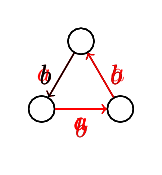
\begin{tikzpicture}
            \graphbox{\( \)}{0mm}{0mm}{20mm}{20mm}{-5mm}{-14mm}{
                \node[draw,circle] (x) at (0,0) {};
                \node[draw,circle] (y) at (1,0) {};
                \node[draw,circle] (z) at (0.5,0.86) {};
                \draw[->,red] (x) -- node[midway,below] {$a$} (y) ;
                \draw[->,red] (y) -- node[midway,right] {$b$} (z) ;
                \draw[->] (z) -- node[midway,left] {$b$} (x) ;
            } 
            \graphbox{\( \)}{22mm}{0mm}{20mm}{20mm}{-5mm}{-14mm}{
                \node[draw,circle] (x) at (0,0) {};  
                \node[draw,circle] (y) at (1,0) {};
                \node[draw,circle] (z) at (0.5,0.86) {};
                \draw[->] (x) -- node[midway,below] {$b$} (y) ;
                \draw[->,red] (y) -- node[midway,right] {$a$} (z) ;
                \draw[->,red] (z) -- node[midway,left] {$b$} (x) ;
            }
            \graphbox{\( \)}{44mm}{0mm}{20mm}{20mm}{-5mm}{-14mm}{
                \node[draw,circle] (x) at (0,0) {};   
                \node[draw,circle] (y) at (1,0) {};
                \node[draw,circle] (z) at (0.5,0.86) {};
                \draw[->,red] (x) -- node[midway,below] {$a$} (y) ;
                \draw[->,red] (y) -- node[midway,right] {$b$} (z) ;
                \draw[->] (z) -- node[midway,left] {$b$} (x) ;
            } 
            \graphbox{\( \)}{66mm}{0mm}{20mm}{20mm}{-5mm}{-14mm}{
                \node[draw,circle] (x) at (0,0) {};  
                \node[draw,circle] (y) at (1,0) {};
                \node[draw,circle] (z) at (0.5,0.86) {};
                \draw[->,red] (x) -- node[midway,below] {$b$} (y) ;
                \draw[->] (y) -- node[midway,right] {$b$} (z) ;
                \draw[->,red] (z) -- node[midway,left] {$a$} (x) ;
            }
            \graphbox{\( \)}{88mm}{0mm}{20mm}{20mm}{-5mm}{-14mm}{
                \node[draw,circle] (x) at (0,0) {};   
                \node[draw,circle] (y) at (1,0) {};
                \node[draw,circle] (z) at (0.5,0.86) {};
                \draw[->,red] (x) -- node[midway,below] {$a$} (y) ;
                \draw[->,red] (y) -- node[midway,right] {$b$} (z) ;
                \draw[->] (z) -- node[midway,left] {$b$} (x) ;
            }
         \end{tikzpicture}
        }
        %  \caption{Sequence of rewriting steps, to be read left to right. In each graph, the subgraph to be replaced to obtain the next graph is highlighted in red.}
        %   \label{fig:preliminaries:sequence_of_transformation_infinite}
        \end{figure}
\end{example}

For a set of rewriting rules \(\mathcal{R}\) (and a DPO rewriting framework \(\mathfrak{F}\)), the impossibility of transforming any object indefinitely with the non-deterministic strategy \enquote{apply rules as long as possible} using rules from \(\mathcal{R}\) (in the framework \(\mathfrak{F}\)) is called \emph{termination}~\cite{middeldorp1997simple}. This property corresponds to program termination on all inputs in conventional programming languages, and is undecidable in general~\cite{plump1998terminationundecidable}.

For example of a non-terminating rule set, consider the set consisting of the rule and the infinite rewriting chain in Example~\ref{example:preliminaries:dggdfgnkfsjksfkjsf}.
% set with the rule and the infinite rewriting chain shown in Figure~\ref{fig:preliminaries:sequence_of_transformation_infinite}. 
For example of a terminating rule set, consider the set with the unique rule, shown below,
% in Figure~\ref{fig:intro:edge_deletion_andffsfjsssdkdsglkadjl}, 
which deletes an edge. 
    \begin{center}
     \resizebox{\textwidth}{!}{ 
                \begin{tikzpicture}[baseline=-3ex]
                    \graphbox{\( L \)}{0mm}{-3mm}{34mm}{15mm}{2mm}{2mm}{
                        \coordinate (o) at (0mm,-11mm); 
                        \node[draw,circle] (l1) at ($(o)+(-10mm,0mm)$) {1};
                        \node[draw,circle] (l2) at ($(l1)+(2,0)$) {2};
                        % \node[draw,circle] (l3) at ($(l1)+(1,0)$) {3};
                        \draw[->] (l1) -- (l2) node[midway,above] {$a$};
                    } 
            
                    \graphbox{\( K \)}{40mm}{-3mm}{34mm}{15mm}{2mm}{2mm}{
                        \coordinate (o) at (0mm,-11mm); 
                        \node[draw,circle] (l1) at ($(o)+(-10mm,0mm)$) {1};
                        \node[draw,circle] (l2) at ($(l1)+(2,0)$) {2};
                    }  
            
                    \graphbox{\( R \)}{80mm}{-3mm}{35mm}{15mm}{2mm}{2mm}{
                        \coordinate (o) at (-5mm,-11mm); 
                        \node[draw,circle] (l1) at ($(o)+(-10mm,0mm)$) {1};
                        % \node[draw,circle] (l2) at ($(l1)+(3,0)$) {2};
                        % \node[draw,circle] (l3) at ($(l1)+(1,0)$) {4};
                        \node[draw,circle] (l4) at ($(l1)+(2,0)$) {2};
                        \draw[->] (l1) -- (l4) node[midway,above] {$b$};
                        % \draw[->] (l4) -- (l2) node[midway,above] {$a$};
                    }    
                    \node () at (37mm,-10mm) {\( \leftarrowtail \)}; % K -> L
                    \node () at (77mm,-10mm) {\( \rightarrowtail \)}; % K -> R
                \end{tikzpicture}
                }
            \end{center}
Any rewriting chain using this rule is finite, because each rewriting step decreases the number of edges by one and a graph has only a finite number of edges by definition.

However, in many cases, an interesting property can be proved even if the whole rule set is not terminating. 
Take the system with rules $\alpha$ and $\beta$ shown below. Rule~$\alpha$ removes one edge per application; rule~$\beta$ introduces a new node. 
\begin{center}
        $\alpha$ = {
             \resizebox{0.9\textwidth}{!}{
             \begin{tikzpicture}[baseline=-7ex]
                    \graphbox{\( \mathcal{L} \)}{0mm}{-3mm}{34mm}{15mm}{2mm}{2mm}{
                        \coordinate (o) at (0mm,-11mm); 
                        \node[draw,circle] (l1) at ($(o)+(-10mm,0mm)$) {$1$};
                        \node[draw,circle] (l2) at ($(l1)+(2,0)$) {$2$};
                        \draw[->] (l1) -- (l2) node[midway,above] {};
                    } 
            
                    \graphbox{\( \mathcal{K} \)}{40mm}{-3mm}{34mm}{15mm}{2mm}{2mm}{
                        \coordinate (o) at (0mm,-11mm); 
                        \node[draw,circle] (l1) at ($(o)+(-10mm,0mm)$) {$1$};
                        \node[draw,circle] (l2) at ($(l1)+(2,0)$) {$2$};
                    }  
            
                    \graphbox{\( \mathcal{R} \)}{80mm}{-3mm}{35mm}{15mm}{5mm}{2mm}{
                        \coordinate (o) at (-5mm,-11mm); 
                        \node[draw,circle] (l1) at ($(o)+(-10mm,0mm)$) {$1$};
                        \node[draw,circle] (l4) at ($(l1)+(2,0)$) {$2$};
                    }    
                    \node () at (37mm,-10mm) {\( \leftarrowtail \)}; % K -> L
                    \node () at (77mm,-10mm) {\( \rightarrowtail \)}; % K -> R
                \end{tikzpicture}
            }
        }
    %     \caption{A graph transformation rule for edge deletion}
    % \label{fig:intro:edge_deletion_rule}
    % \end{subfigure}
    
    % \begin{subfigure}{0.3\textwidth}
    %     % \centering

        $\beta$ ={
             \resizebox{0.9\textwidth}{!}{
             \begin{tikzpicture}[baseline=-7ex]
                    \graphbox{\( \mathcal{L} \)}{0mm}{-3mm}{34mm}{15mm}{2mm}{2mm}{
                        
                    } 
            
                    \graphbox{\( \mathcal{K} \)}{40mm}{-3mm}{34mm}{15mm}{2mm}{2mm}{
                       
                    }  
            
                    \graphbox{\( \mathcal{R} \)}{80mm}{-3mm}{35mm}{15mm}{5mm}{2mm}{
                        \coordinate (o) at (0mm,-11mm); 
                        \node[draw,circle] (l1) at ($(o)+(-10mm,0mm)$) {};
                    }    
                    \node () at (37mm,-10mm) {\( \leftarrowtail \)}; % K -> L
                    \node () at (77mm,-10mm) {\( \rightarrowtail \)}; % K -> R
                \end{tikzpicture}
            }
        }
    %     \caption{A graph transformation rule for node addition}
    %     \label{fig:intro:node_addition_rule}
    % \end{subfigure} 
            \end{center}
Because $\beta$ can always be re-applied to generate additional nodes, infinite rewriting sequences exist. Conversely, $\alpha$ is applicable only 
a finite number of times in any rewriting chain, since each application removes an edge and no rule adds edges. Since the initial graph is finite, the possibility of non-termination stems exclusively from $\beta$. This attribution illustrates the broader idea of \emph{relative termination} as introduced by Klop~\cite{klop1987term} and explored in~\cite{geser1990relative,kassing2024dependency,endrullis2024generalized_icgt,zantema2014termination,bruggink2014termination,bruggink2015proving}.
\begin{definition}
Let $A$ be a collection of objects and let $R$ and $S$ be binary relations on $A$. 
We say that $R$ is \textbf{terminating relative to} $S$ (or that $R$ \textbf{terminates relative to} $S$) if 
any $(R \mathop{\cup} S)$-chain contains only a finite number of $R$-steps.
In particular, $R$ is \textbf{terminating} (or terminates) if it is terminating relative to the empty relation $\emptyset$.
\end{definition}

For example, the relation $>$ on $\mathbb{N}$ is terminating relative to the empty relation, since any $(\mathop{>} \mathop{\cup} \emptyset)$-chain contains only a finite number of $>$-steps. The relation $>$ is also terminating relative to $\geq$ on $\mathbb{N}$, since any $(\mathop{>} \mathop{\cup} \mathop{\geq})$-chain can only contain a finite number of $>$-steps.

% Note that termination and well-foundedness are the same property of a binary relation $\to$ described from two perspectives. Operationally, we read $x \mathop{\to} y$ as \enquote{$x$ can be transformed to $y$}; the absence of infinite $\rightarrow$-chains therefore means that any transformation sequence starting from an initial object $x$ is finite, i.e. every computation or rewrite sequence eventually terminates. Structurally, we read $x \mathop{\to} y$ as \enquote{$x$ is constructed from $y$}; the absence of infinite $\to$-chains then implies that every object $x$ can be traced back along a finite chain to an element that is not constructed from any other, so the structure is well-founded. In this thesis we adopt the operational viewpoint and use the term termination.

Relative termination 
carries over to rewriting systems in a straightforward way via their associated rewriting relations.
\begin{definition}
    \label{termination:def:relative_termination}
     Let $\mathcal{R}$ and $\mathcal{S}$ be sets of rewriting rules and let $\mathfrak{F}$ be a DPO rewriting framework. 
     We say that $\mathop{\Rightarrow}_{\mathcal{R},\mathfrak{F}}$ is \textbf{terminating relative to} $\mathop{\Rightarrow}_{\mathcal{S}, \mathfrak{F}}$ if 
     $\mathop{\Rightarrow}_{\mathcal{R},\mathfrak{F}}$ is \textbf{terminating relative to} $\mathop{\Rightarrow}_{\mathcal{S}, \mathfrak{F}}$.
\end{definition}
In practice, to prove termination of a rewriting system $\mathcal{R}$, one partitions the set of rules into two disjoint subsets \( \mathcal{B} \) and \( \mathcal{A} \) with non-empty $\mathcal{A}$ such that \( \mathcal{A} \) terminates relative to \( \mathcal{B} \). 
If $\mathcal{B}$ is empty then the termination of $\mathcal{R}$ is established, otherwise, a new iteration starts with the strictly smaller rule set $\mathcal{B}$.
 